% This must be in the first 5 lines to tell arXiv to use pdfLaTeX, which is strongly recommended.
\pdfoutput=1
% In particular, the hyperref package requires pdfLaTeX in order to break URLs across lines.

\documentclass[11pt]{article}

% Remove the "review" option to generate the final version.
\usepackage{acl}

% Standard package includes
\usepackage{times}
\usepackage{latexsym}
\usepackage{inconsolata}
\usepackage{amsfonts}
\usepackage{soul}
\usepackage{colortbl}
\usepackage{multirow}
\usepackage{xspace}
\usepackage{amsmath}
\usepackage{graphicx}
\usepackage{booktabs}


\newcommand{\biasbranch}{bias-only branch\xspace}
\newcommand{\originalbranch}{original branch\xspace}
\newcommand{\mc}[2]{\multicolumn{#1}{c}{#2}}
\newcommand{\swap}[3][-]{#3#1#2} 
\newcommand{\std}[1]{{\scriptsize{$\pm$#1}}}
\newcommand{\xhdr}[1]{\vspace{0em}\noindent{{\bf #1.}}}
\newcommand{\na}{~~~~~~~N/A~~~~~~~~}

\newcommand{\FT}{\textsc{FineTune}\xspace}
\newcommand{\MASK}{\textsc{DebiasMask}\xspace}
\newcommand{\KW}{\textsc{KernelWhitening}\xspace}
\newcommand{\ETE}{\textsc{E2E-PoE}\xspace}
\newcommand{\etefocal}{\textsc{E2E-Focal}\xspace}
\newcommand{\RUBI}{\textsc{RUBi}\xspace}
\newcommand{\IE}{\textsc{IEGDB}\xspace}
\newcommand{\READ}{\textsc{READ}\xspace}
\newcommand{\OursName}{\textsc{FairFlow}\xspace}
\newcommand{\OursPoe}{\OursName-\textsc{poe}\xspace}
\newcommand{\OursFocal}{\OursName-\textsc{focal}\xspace}
% \newcommand{\OursCL}{\OursName-\textsc{cl}\xspace}
\newcommand{\OursCL}{\OursName}

\newcommand{\jiali}[1]{{\color{blue}[[J: #1]]}}
\newcommand{\hadi}[1]{{\color{orange}[H: #1]}}

% For proper rendering and hyphenation of words containing Latin characters (including in bib files)
\usepackage[T1]{fontenc}
% For Vietnamese characters
% \usepackage[T5]{fontenc}
% See https://www.latex-project.org/help/documentation/encguide.pdf for other character sets

% This assumes your files are encoded as UTF8
\usepackage[utf8]{inputenc}

% This is not strictly necessary and may be commented out.
% However, it will improve the layout of the manuscript,
% and will typically save some space.
\usepackage{microtype}

% This is also not strictly necessary and may be commented out.
% However, it will improve the aesthetics of text in
% the typewriter font.
\usepackage{inconsolata}


% If the title and author information does not fit in the area allocated, uncomment the following
%
%\setlength\titlebox{<dim>}
%
% and set <dim> to something 5cm or larger.

% \title{Contrastive-based Multiview Dataset Bias Mitigation for Natural Language Processing}
\title{\OursName: Mitigating Dataset Biases through Undecided Learning\\for Natural Language Understanding} %: A Multiview Contrastive Framework for Robust Debiasing

% Author information can be set in various styles:
% For several authors from the same institution:
% \author{Author 1 \and ... \and Author n \\
%         Address line \\ ... \\ Address line}
% if the names do not fit well on one line use
%         Author 1 \\ {\bf Author 2} \\ ... \\ {\bf Author n} \\
% For authors from different institutions:
% \author{Author 1 \\ Address line \\  ... \\ Address line
%         \And  ... \And
%         Author n \\ Address line \\ ... \\ Address line}
% To start a separate ``row'' of authors use \AND, as in
% \author{Author 1 \\ Address line \\  ... \\ Address line
%         \AND
%         Author 2 \\ Address line \\ ... \\ Address line \And
%         Author 3 \\ Address line \\ ... \\ Address line}

\author{Jiali Cheng \and Hadi Amiri \\
  University of Massachusetts Lowell \\
  \texttt{\{jiali\_cheng, hadi\_amiri\}@uml.edu}
\\}

\begin{document}
\maketitle



Inference scaling empowers LLMs with unprecedented reasoning ability, with reinforcement learning as the core technique to elicit complex reasoning. However, key technical details of state-of-the-art reasoning LLMs are concealed (such as in OpenAI o1 blog and DeepSeek R1 technical report), thus the community still struggles to reproduce their RL training results.
We propose the \textbf{D}ecoupled Clip and \textbf{D}ynamic s\textbf{A}mpling \textbf{P}olicy \textbf{O}ptimization (\method) algorithm, and fully open-source a state-of-the-art large-scale RL system that achieves 50 points on AIME 2024 using Qwen2.5-32B base model.
Unlike previous works that withhold training details, we introduce four key techniques of our algorithm that make large-scale LLM RL a success. In addition, we open-source our training code, which is built on the \textbf{verl} framework~\footnote{\url{https://github.com/volcengine/verl}}, along with a carefully curated and processed dataset. These components of our open-source system enhance reproducibility and support future research in large-scale LLM RL.

% \qiying{Comment like this}

% \hao{Comment like this}

% \zheng{Comment like this}

% \weinan{Comment like this}

% \hongli{Comment like this}
\vspace{-20pt}
\begin{figure}[h]
    \centering
    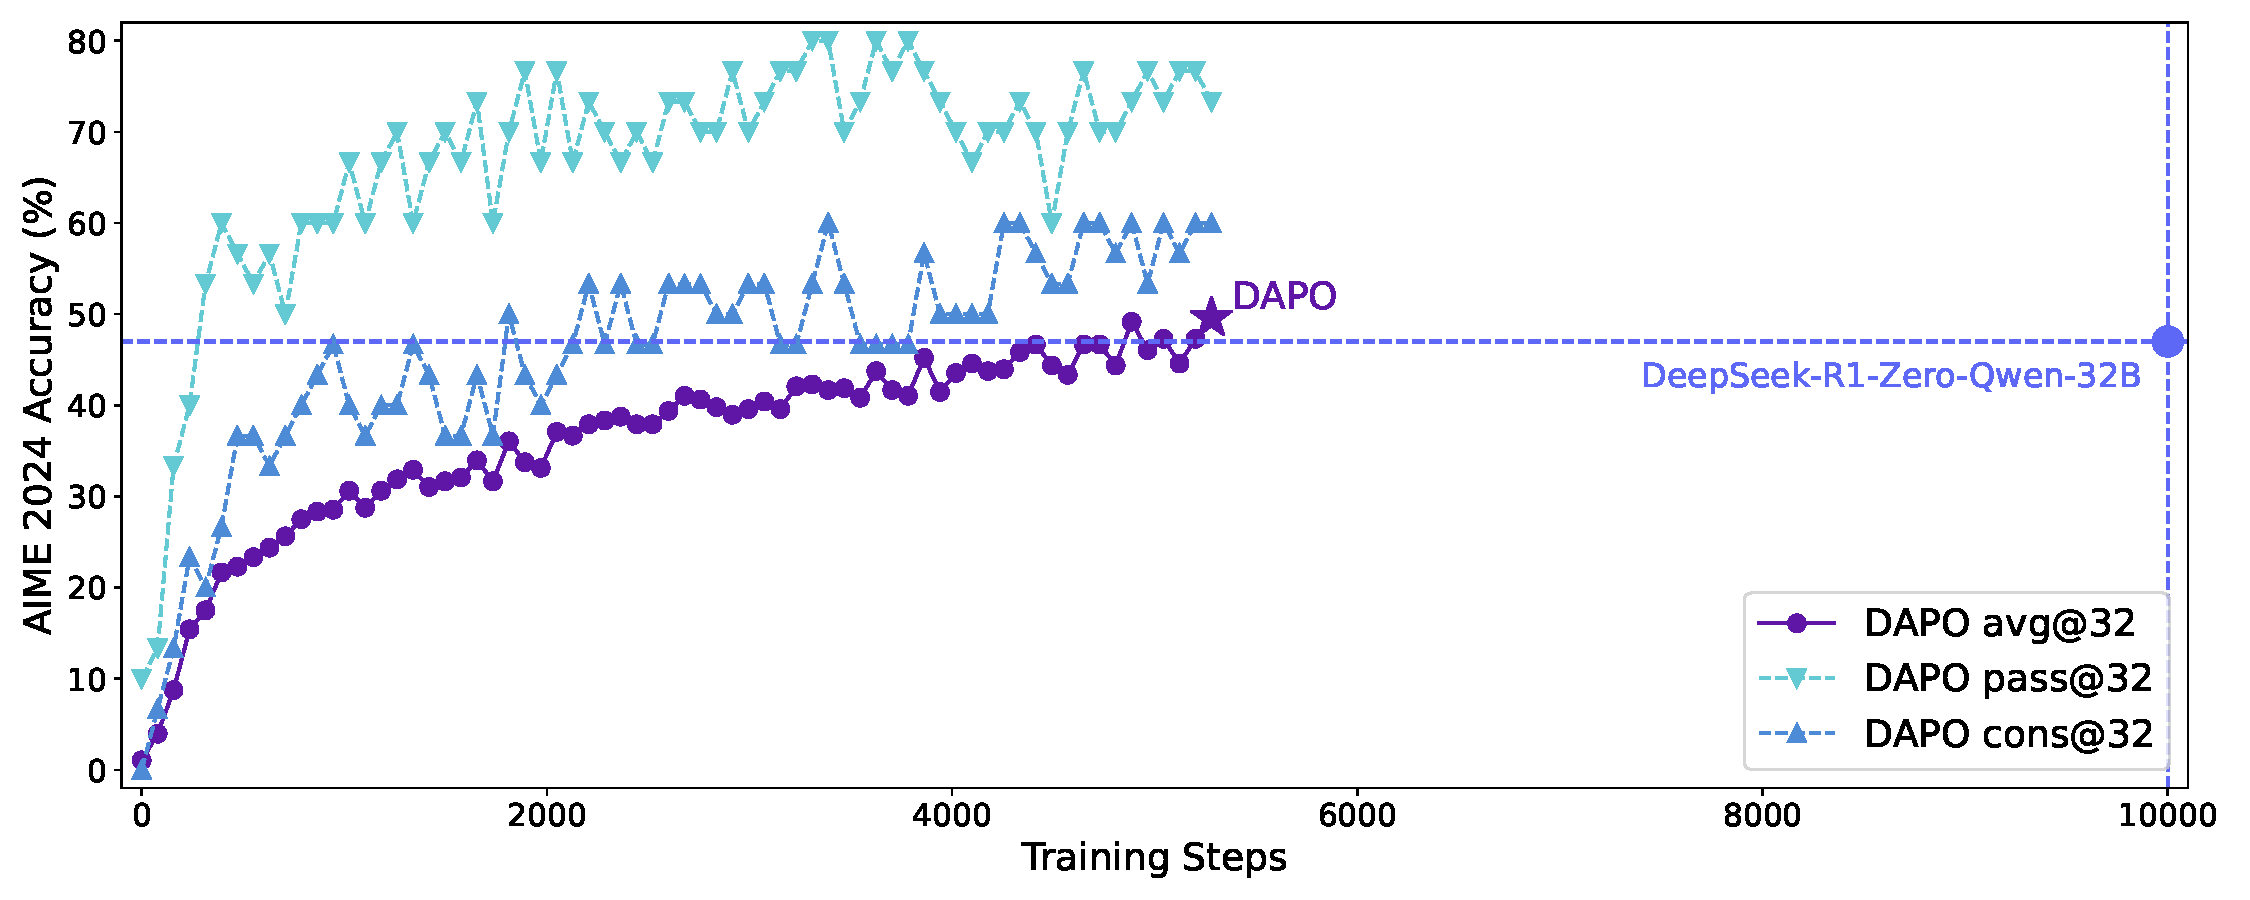
\includegraphics[width=0.92\linewidth]{figures/score.pdf}
    \caption{AIME 2024 scores of \method on the Qwen2.5-32B base model, outperforming the previous SoTA DeepSeek-R1-Zero-Qwen-32B using 50\% training steps.}
    \label{fig:front}
\end{figure}

\newpage
\section{Introduction}

Test-time scaling such as OpenAI's o1~\cite{o1} and DeepSeek's R1~\cite{guo2025deepseek} brings a profound paradigm shift to Large Language Models (LLMs)~\cite{gpt4,claude35sonnet,gpt3,chowdhery2023palm,dsv3}. Test-time scaling enables longer Chain-of-Thought thinking and induces sophisticated reasoning behaviors, which makes the models superior in competitive math and coding tasks like AIME and Codeforces.

The central technique driving the revolution is large-scale Reinforcement Learning (RL), which elicits complex reasoning behaviors such as self-verification and iterative refinement. However, the actual algorithm and key recipe for scalable RL training remains a myth, hidden from technical reports of existing reasoning models~\cite{o1,guo2025deepseek,grok,gemini-thinking,qwq,k1.5}. In this paper, we reveal significant obstacles in large-scale RL training and open-source a scalable RL system with fully open-sourced algorithm, training code and dataset that provides democratized solutions with industry-level RL results. 

We experiment over Qwen2.5-32B~\cite{yang2024qwen2} as the pretrained model for RL. In our initial GRPO run, we achieved only 30 points on AIME — a performance significantly below DeepSeek’s RL (47 points). A thorough analysis reveals that the naive GRPO baseline suffers from several key issues such as entropy collapse, reward noise, and training instability. The broader community has encountered similar challenges in reproducing DeepSeek's results~\cite{rendarl,OpenReasonerZero2025,hu2025reinforce++,cui2025process,lee2024token,kazemnejad2024vineppo,yuan2025s} suggesting that critical training details may have been omitted in the R1 paper that are required to develop an industry-level, large-scale, and reproducible RL system.

To close this gap, we release an open-source state-of-the-art system for large-scale LLM RL, which achieves 50 points on AIME 2024 based on Qwen2.5-32B model, outperforming previous state-of-the-art results achieved by DeepSeek-R1-Zero-Qwen-32B~\cite{guo2025deepseek} (47 points) using 50\% training steps (Figure~\ref{fig:front}). We propose the \textbf{D}ecoupled Clip and \textbf{D}ynamic s\textbf{A}mpling \textbf{P}olicy \textbf{O}ptimization (\textbf{DAPO}) algorithm, and introduce 4 key techniques to make RL shine in the long-CoT RL scenario. Details are presented in Section~\ref{sec:method}.
\begin{enumerate}
    \item \textbf{Clip-Higher}, which promotes the diversity of the system and avoids entropy collapse;
    \item \textbf{Dynamic Sampling}, which improves training efficiency and stability;
    \item \textbf{Token-Level Policy Gradient Loss}, which is critical in long-CoT RL scenarios;
    \item \textbf{Overlong Reward Shaping}, which reduces reward noise and stabilizes training.
\end{enumerate}
Our implementation is based on verl~\cite{sheng2024hybridflow}. By fully releasing our state-of-the-art RL system including training code and data, we aim to reveal valuable insights to large-scale LLM RL that benefit the larger community.

\section{DAPO}
\label{sec:method}

We propose the \textbf{D}ecouple Clip and \textbf{D}ynamic s\textbf{A}mpling \textbf{P}olicy \textbf{O}ptimization (DAPO) algorithm. DAPO samples a group of outputs $\{o_i\}_{i=1}^G$ for each question $q$ paired with the answer $a$, and optimizes the policy via the following objective:
\begin{equation}
\begin{aligned}
\mathcal{J}_{\text{DAPO}}(\theta) =\quad& \mathbb{E}_{(q,a)\sim \mathcal{D}, \{o_i\}_{i=1}^G\sim \pi_{\theta_\text{old}}(\cdot\mid q)}\\&
\Bigg[\frac{1}{\sum_{i=1}^{G}|o_i|}\sum_{i=1}^{G}\sum_{t=1}^{|o_i|} 
\min \Big( r_{i,t}(\theta) \hat{A}_{i,t},  
\ \text{clip} \Big( r_{i,t}(\theta), 1 - {\varepsilon_{\text{low}}}, 1 + {\varepsilon_{\text{high}}} \Big) \hat{A}_{i,t} \Big) \Bigg]
\\
\text{s.t.}\quad& 0< \Big|\{o_i\mid\texttt{is\_equivalent}(a,o_i)\}\Big|< G,
\label{eq:dapoloss}
\end{aligned}
\end{equation}
where
\begin{equation}
    r_{i,t}(\theta)=\frac{\pi_{\theta}(o_{i,t} \mid q, o_{i,<t})}{\pi_{\theta_{\text{old}}}(o_{i,t} \mid q,o_{i,<t})},\quad\hat{A}_{i,t} = \frac{R_i - \text{mean}(\{R_i\}_{i=1}^G)}{\text{std}(\{R_i\}_{i=1}^G)}.
\label{eq:advantage_calculation}
\end{equation}
The full algorithm can be found in Algorithm~\ref{algo:dapo}. In this section, we will introduce the key techniques associated with DAPO.

\subsection{Raise the Ceiling: Clip-Higher}
\label{sec:cliphigher}

In our initial experiments using naive PPO~\cite{schulman2017proximal} or GRPO~\cite{deepseekmath}, we observed the entropy collapse phenomenon: the entropy of the policy decreases quickly as training progresses (\Cref{fig:cliphigh_entropy}). The sampled responses of certain groups tend to be nearly identical. This indicates limited exploration and early deterministic policy, which can hinder the scaling process. 

We propose the \textbf{Clip-Higher} strategy to address this issue. Clipping over the importance sampling ratio is introduced in Clipped Proximal Policy Optimization (PPO-Clip)~\cite{schulman2017proximal} to restrict the trust region and enhance the stability of RL. 
We identify that the upper clip can restrict the exploration of the policy. In this case, it is much easier to make an `exploitation token' more probable, than to uplift the probability of an unlikely `exploration token'.

Concretely, when $\varepsilon = 0.2$ (the default value of most algorithms), consider two actions with probabilities $\pi_{\theta_{\text{old}}}(o_i \mid q) = 0.01$ and $0.9$. The maximum possible updated probabilities $\pi_{\theta}(o_i \mid q)$ are $0.012$ and $1.08$, respectively. 
This implies that for tokens with a higher probability (\eg, 0.9) is less constrained. Conversely, for low-probability tokens, achieving a non-trivial increase in probability is considerably more challenging.
Empirically, we also observe that the maximum probability of clipped tokens is approximately $\pi_{\theta}(o_i \mid q) < 0.2$ (\Cref{fig:max_prob_clipped}). This finding supports our analysis that the upper clipping threshold indeed restricts the probability increase of low-probability tokens, thereby potentially constraining the diversity of the system.

Adhering to the \textbf{Clip-Higher} strategy, we decouple the lower and higher clipping range as $\varepsilon_\text{low}$ and $\varepsilon_\text{high}$, as highlighted in Equation~\ref{eq:dapoloss_clip_higher}:
\begin{equation}
\begin{aligned}
\mathcal{J}_{\text{DAPO}}(\theta) = \quad&\mathbb{E}_{(q,a)\sim\mathcal{D}, \{o_i\}_{i=1}^G\sim \pi_{\theta_\text{old}}(\cdot\mid q)}\\&
\Bigg[\frac{1}{\sum_{i=1}^{G}|o_i|}\sum_{i=1}^{G}\sum_{t=1}^{|o_i|} 
\min \Big( r_{i,t}(\theta) \hat{A}_{i,t},  
\ \text{clip} \Big( r_{i,t}(\theta), 1 - {\color{red}\varepsilon_{\text{low}}}, 1 + {\color{red}\varepsilon_{\text{high}}} \Big) \hat{A}_{i,t} \Big) \Bigg]\\
\text{s.t.}\quad& 0< \Big|\{o_i\mid\texttt{is\_equivalent}(a,o_i)\}\Big|< G.
\label{eq:dapoloss_clip_higher}
\end{aligned}
\end{equation}
We increase the value of \( \varepsilon_{\text{high}} \) to leave more room for the increase of low-probability tokens. As shown in \Cref{fig:clip_high}, this adjustment effectively enhances the policy's entropy and facilitates the generation of more diverse samples.
We opt to keep \( \varepsilon_{\text{low}} \) relatively small, because increasing it will suppress the probability of these tokens to $0$, resulting in the collapse of the sampling space.

% \begin{figure}[h]
%     \centering
%     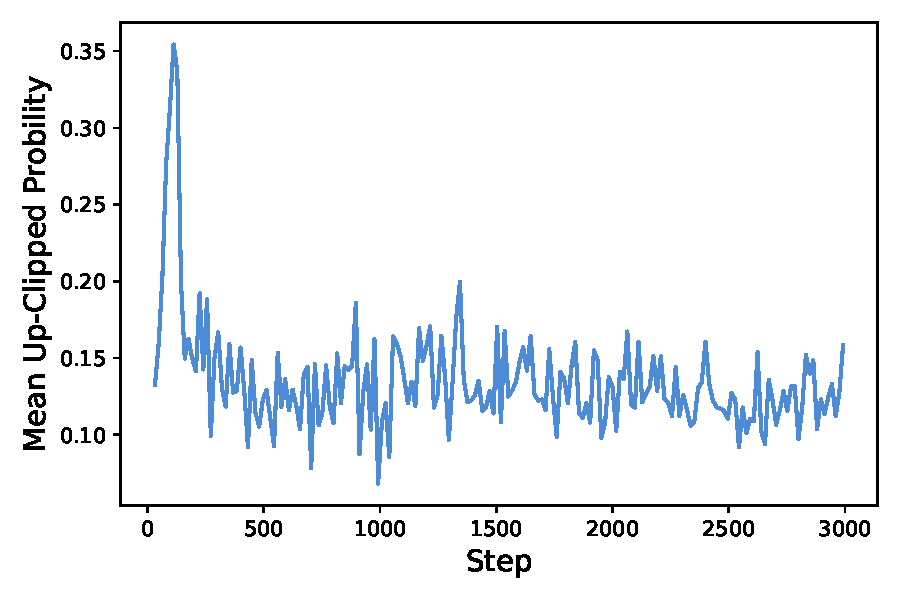
\includegraphics[width=0.5\linewidth]{figures/3.1.3.pdf}
%     \caption{Maximum clipped probabilities.}
%     \label{fig:max_prob_clipped}
% \end{figure}

% \begin{figure}[h]
%     \centering
%     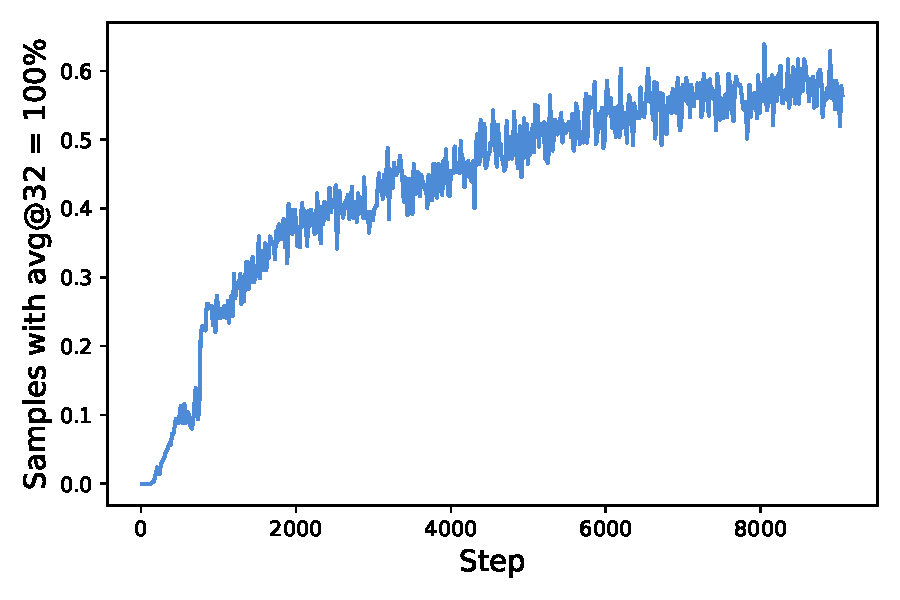
\includegraphics[width=0.5\textwidth]{figures/3.2.1.pdf}
%     \caption{The proportion of samples with an accuracy of 1 during the RL training process.}
%     \label{fig:num_samples_eq_1}
% \end{figure}

\begin{figure}
    \centering
    \begin{subfigure}{0.49\textwidth}
        \centering
        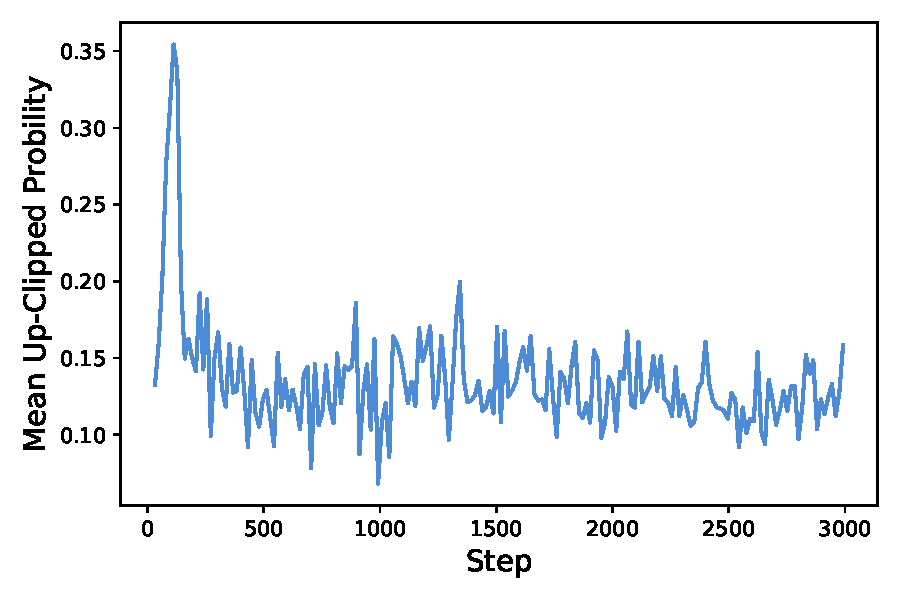
\includegraphics[width=\textwidth]{figures/3.1.3.pdf}
        \caption{Maximum clipped probabilities.}
        \label{fig:max_prob_clipped}
    \end{subfigure}
    \hfill
    \begin{subfigure}{0.49\textwidth}
        \centering
        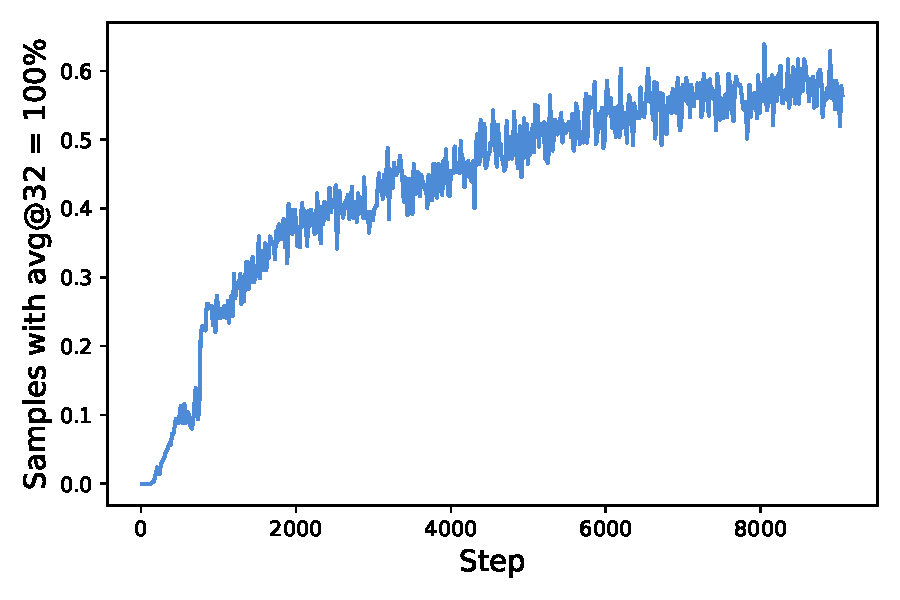
\includegraphics[width=\textwidth]{figures/3.2.1.pdf}
    \caption{The proportion of samples with an accuracy of 1.}
    \label{fig:num_samples_eq_1}
    \end{subfigure}
    
    \caption{The entropy of the probability distribution of the actor model, as well as the changes in response length.}
    \label{fig:3212}
\end{figure}

\subsection{The More the Merrier: Dynamic Sampling}
\label{sec:gradientkeeping}

Existing RL algorithm suffers from the gradient-decreasing problem when some prompts have accuracy equal to 1. For example for GRPO, if all outputs $\{o_i\}_{i=1}^G$ of a particular prompt are correct and receive the same reward 1, the resulting advantage for this group is \textit{zero}. A zero advantage results in no gradients for policy updates, thereby reducing sample efficiency. Empirically, the number of samples with accuracy equal to 1 continues to increase, as shown in \Cref{fig:num_samples_eq_1}. This means that the effective number of prompts in each batch keeps decreasing, which can lead to larger variance in gradient and dampens the gradient signals for model training.

To this end, we propose to \textbf{over-sample and filter out prompts with the accuracy equal to 1 and 0} illustrated in Equation~\ref{eq:dapoloss_oversample_filter}, leaving all prompts in the batch with effective gradients and keeping a consistent number of prompts. Before training, we keep sampling until the batch is fully filled with samples whose accuracy is neither 0 nor 1.

\begin{equation}
\begin{aligned}
\mathcal{J}_{\text{DAPO}}(\theta) =\quad& \mathbb{E}_{(q,a)\sim \mathcal{D}, \{o_i\}_{i=1}^G\sim \pi_{\theta_\text{old}}(\cdot\mid q)}\\&
\Bigg[\frac{1}{\sum_{i=1}^{G}|o_i|}\sum_{i=1}^{G}\sum_{t=1}^{|o_i|} 
\min \Big( r_{i,t}(\theta) \hat{A}_{i,t},  
\ \text{clip} \Big( r_{i,t}(\theta), 1 - {\varepsilon_{\text{low}}}, 1 + {\varepsilon_{\text{high}}} \Big) \hat{A}_{i,t} \Big) \Bigg]
\\
\text{s.t.}\quad& {\color{red}0< \Big|\{o_i\mid\texttt{is\_equivalent}(a,o_i)\}\Big|< G}.
\label{eq:dapoloss_oversample_filter}
\end{aligned}
\end{equation}

Note that this strategy does not necessarily impede training efficiency, because the generation time is typically dominated by the generation of long-tail samples if the RL system is synchronized and the generation stage is not pipelined. Besides, we find that with dynamic sampling the experiment achieves the same performance faster as shown in~\Cref{fig:afos_compare}.

% Generally, our strategy serves as a filter that screens every group of outputs and discards those rewarded with minimum or maximum scores, as these extreme samples are more likely to cluster and produce zero gradients. 
% However, a straightforward filtering approach can undermine training stability because the proportion of extreme samples varies across different batches, resulting in inconsistent numbers of useful samples at each training step. 
% To address this issue, we employ an up-sampling strategy for useful responses until the batch is fully filled. 
% Specifically, we repeat the sampling process for each prompt $q$, and subsequently discard extreme samples until the remaining samples fill the original batch size.


\subsection{Rebalancing Act: Token-Level Policy Gradient Loss}
\label{sec:tokenlevel}

The original GRPO algorithm employs a sample-level loss calculation, which involves first averaging the losses by token within each sample and then aggregating the losses across samples. In this approach, each sample is assigned an equal weight in the final loss computation. However, we find that this method of loss reduction introduces several challenges in the context of long-CoT RL scenarios.

Since all samples are assigned the same weight in the loss calculation,  tokens within longer responses (which contain more tokens) may have a disproportionately lower contribution to the overall loss, which can lead to two adverse effects.
First, for high-quality long samples, this effect can impede the model's ability to learn reasoning-relevant patterns within them.
Second, we observe that excessively long samples often exhibit low-quality patterns such as gibberish and repetitive words. Thus, sample-level loss calculation, due to its inability to effectively penalize those undesirable patterns in long samples, leads to an unhealthy increase in entropy and response length, as shown in 
\Cref{fig:token_loss_entropy} and \Cref{fig:token_loss_length}.

\begin{figure}
    \centering
    \begin{subfigure}{0.49\textwidth}
        \centering
        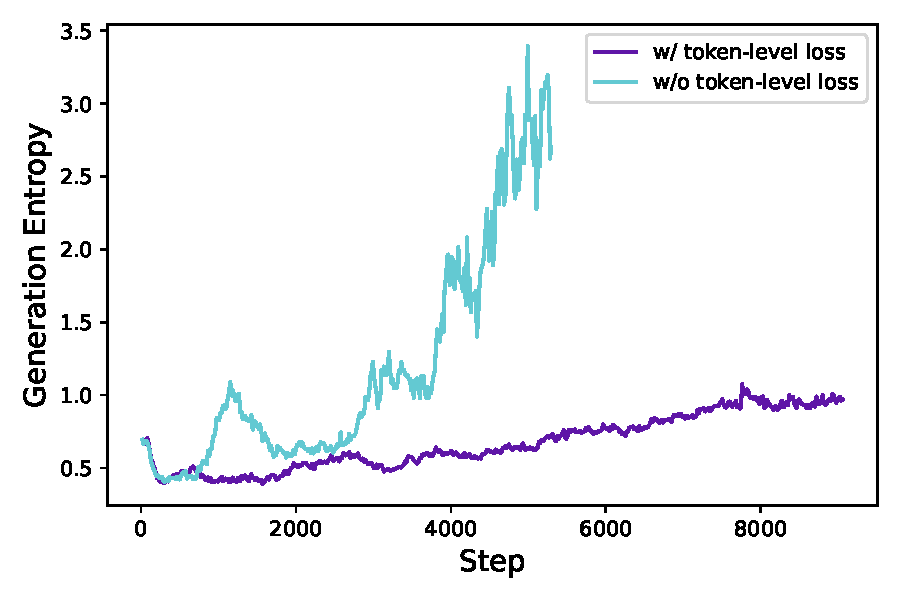
\includegraphics[width=\textwidth]{figures/3.3.1.pdf}
        \caption{Entropy of actor model's generation probabilities.}
        \label{fig:token_loss_entropy}
    \end{subfigure}
    \hfill
    \begin{subfigure}{0.49\textwidth}
        \centering
        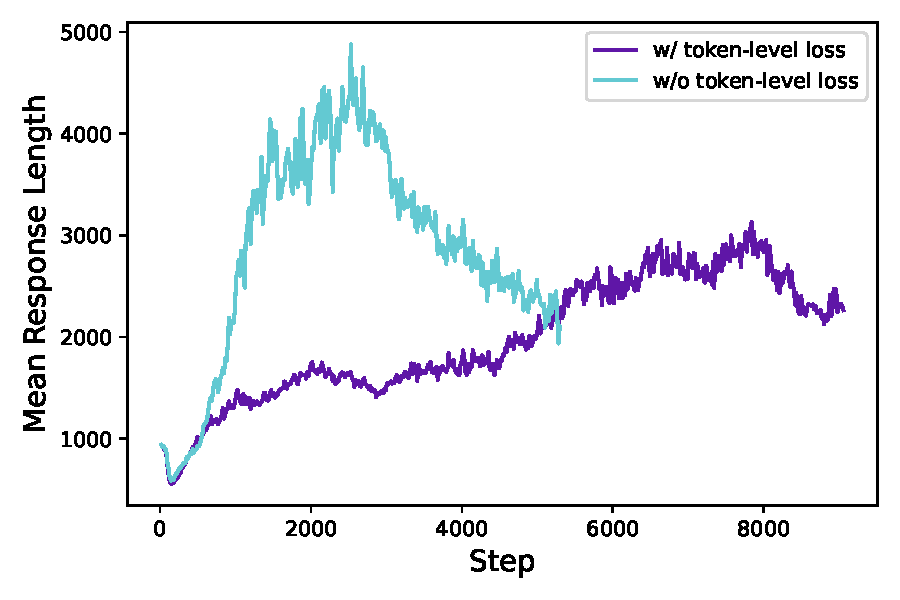
\includegraphics[width=\textwidth]{figures/3.3.2.pdf}
        \caption{Average length of actor model-generated responses}
        \label{fig:token_loss_length}
    \end{subfigure}
    
    \caption{The entropy of the probability distribution of the actor model, as well as the changes in response length.}
    \label{fig:3212}
\end{figure}

We introduce a \textbf{Token-level Policy Gradient Loss} in the long-CoT RL scenario to address the above limitations:
\begin{equation}
\begin{aligned}
\mathcal{J}_{\text{DAPO}}(\theta) = \quad&\mathbb{E}_{(q,a)\sim \mathcal{D}, \{o_i\}_{i=1}^G\sim \pi_{\theta_\text{old}}(\cdot\mid q)}\\&
\Bigg[\frac{1}{\color{red}\sum_{i=1}^{G}|o_i|}{\color{red}\sum_{i=1}^{G}\sum_{t=1}^{|o_i|}} 
\min \Big( r_{i,t}(\theta) \hat{A}_{i,t},  
\ \text{clip} \Big( r_{i,t}(\theta), 1 - {\varepsilon_{\text{low}}}, 1 + {\varepsilon_{\text{high}}} \Big) \hat{A}_{i,t} \Big) \Bigg],\\
\text{s.t.}\quad& 0< \Big|\{o_i\mid\texttt{is\_equivalent}(a,o_i)\}\Big|< G.
\label{eq:dapoloss_token_level_pg_loss}
\end{aligned}
\end{equation}
% Formally, let \( o_i \) denote a response and \( o_{i,t} \) represent the \( t \)-th token in \( o_i \), with the total number of tokens in \( o_i \) given by \( |o_i| \).
In this setting, longer sequences can have more influence on the overall gradient update compared to shorter sequences. 
Moreover, from the perspective of individual tokens, if a particular generation pattern can lead to an increase or decrease in reward, it will be equally prompted or suppressed, regardless of the length of the response in which it appears.
% The new objective function of GRPO can then be expressed as:
% \begin{equation}
% \mathcal{J}(\theta) = \mathbb{E}_{q\sim P(Q), \{o_i\}_{i=1}^G\sim \pi_{\theta_\text{old}}(O\mid q)}
% \Bigg[\frac{1}{\sum_{i=1}^{G}|o_i|}\sum_{i=1}^{G}\sum_{t=1}^{|o_i|} 
% \min \Big( r_{i,t}(\theta) \hat{A}_{i,t},  
% \ \text{clip} \Big( r_{i,t}(\theta), 1 - \varepsilon_{\text{low}}, 1 + \varepsilon_{\text{high}} \Big) \hat{A}_{i,t} \Big) \Bigg].
% \label{eq:token-level-grpo}
% \end{equation}

% \paragraph{Removal of KL Penalty} The KL penalty was originally introduced in reinforcement learning to regulate the divergence between the online policy and the frozen reference policy. In conventional RLHF settings, the goal during the RL phase is to optimize model alignment while preserving the SFT model generation patterns. However, during training of the reasoning model, the output distribution diverges significantly from base model. In this context, the KL regularization term may instead hinder training progress. Our experiments demonstrate that removing the KL penalty from the loss function leads to improved performance.

% \begin{equation}
% \mathcal{J}_{GRPO}(\theta) =
% \frac{1}{G\sum_{i=1}^{G}{|o_i|}} \sum_{i=1}^{G} \sum_{t=1}^{|o_i|} 
% \min \Bigg[
% \frac{\pi_{\theta} (o_{i,t} \mid q, o_{i,<t})}{\pi_{\theta_{old}} (o_{i,t} \mid q, o_{i,<t})} \hat{A}_{i,t}, 
% \operatorname{clip} \Bigg( 
% \frac{\pi_{\theta} (o_{i,t} \mid q, o_{i,<t})}{\pi_{\theta_{old}} (o_{i,t} \mid q, o_{i,<t})}, 1 - \varepsilon, 1 + \varepsilon 
% \Bigg) \hat{A}_{i,t}\Bigg]
% \label{eq:token-level-grpo-our}
% \end{equation}


\subsection{Hide and Seek: Overlong Reward Shaping}
\label{sec:overlong}

In RL training, we typically set a maximum length for generation, with overlong samples truncated accordingly. We find that improper reward shaping for truncated samples can introduce reward noise and significantly disrupt the training process.

By default, we assign a punitive reward to truncated samples.
This approach may introduce noise into the training process, as a sound reasoning process can be penalized solely due to its excessive length. Such penalties can potentially confuse the model regarding the validity of its reasoning process.

\vspace{5pt}
To investigate the impact of this reward noise, we first apply an \textbf{Overlong Filtering} strategy which masks the loss of truncated samples. We find that this approach significantly stabilizes training and enhances performance, as demonstrated in \Cref{fig:overlong_shaping}.

\begin{figure}[t]
    \centering
    \begin{subfigure}{0.49\textwidth}
        \centering
        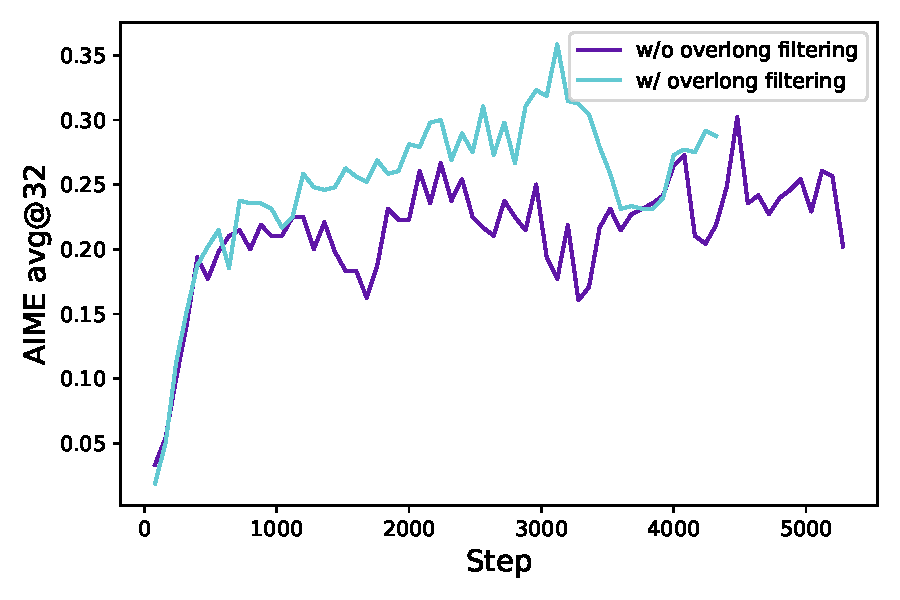
\includegraphics[width=\textwidth]{figures/3.4.1.pdf}
        \caption{Performance on AIME.}
        \label{fig:overlong_acc}
    \end{subfigure}
    \hfill
    \begin{subfigure}{0.49\textwidth}
        \centering
        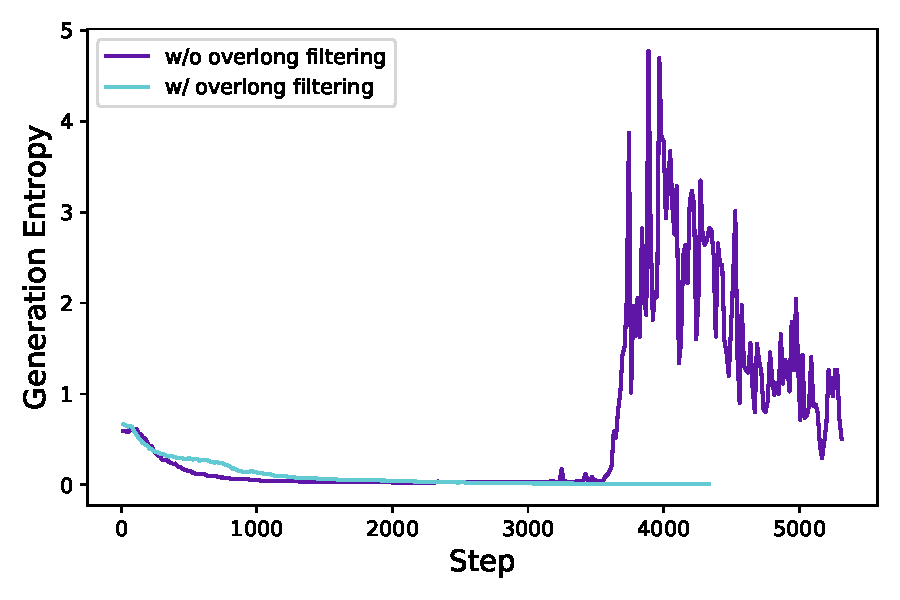
\includegraphics[width=\textwidth]{figures/3.4.2.pdf}
        \caption{Entropy of actor model.}
        \label{fig:overlong_entropy}
    \end{subfigure}
    \caption{The accuracy of the actor model on AIME and the entropy of its generation probabilities, both before and after applying \textbf{Overlong Reward Shaping} strategy.}
    \label{fig:overlong_shaping}
\end{figure}

\setcounter{table}{0}
\begin{table}[h]
    \centering
    \begin{tabular}{@{}p{1.0\textwidth}@{}} 
        \toprule 
        \textbf{Algorithm 1} \; \textbf{DAPO}: \textbf{D}ecoupled Clip and \textbf{D}ynamic s\textbf{A}mpling \textbf{P}olicy \textbf{O}ptimization \\
        \midrule 
        \textbf{Input} initial policy model $\pi_\theta$; reawrd model $R$; task prompts $\mathcal{D}$; hyperparameters $\varepsilon_\mathtt{low}, \varepsilon_\mathtt{high}$ \\
        \;1: \textbf{for} step = 1,...,M \textbf{do} \\
        \;2: \;\;\; Sample a batch $\mathcal{D}_b$ from $\mathcal{D}$ \\
        \;3: \;\;\; Update the old policy model $\pi_{\theta_{old}} \leftarrow \pi_\theta$\\
        \;4: \;\;\; Sample \textit{G} outputs $\{o_i\}_{i=1}^{G} \sim \pi_{\theta_{\text{old}}}(\cdot | q)$ for each question $q \in \mathcal{D}_b$ \\
        \;5: \;\;\; Compute rewards $\{r_i\}_{i=1}^{G}$ for each sampled output $o_i$ by running $R$ \\
        \;6: \;\;\; Filter out $o_i$ and add the remaining to the dynamic sampling buffer (\textbf{Dynamic Sampling} \Cref{eq:dapoloss_oversample_filter})\\
        \;7: \;\;\; \textbf{if} buffer size $n_b<N$: \\
        \;8: \;\;\;\;\;\;\;\; \textbf{continue} \\
            \;9: \;\;\; For each $o_i$ in the buffer, compute $\hat{A}_{i,t}$ for the \textit{t}-th token of $o_i$ (\Cref{eq:advantage_calculation}) \\
        \;10: \;\; \textbf{for} iteration = 1, ..., $\mu$ \textbf{do}\\
        \;11: \;\;\;\;\;\;\; Update the policy model $\pi_\theta$ by maximizing the DAPO objective (\Cref{eq:dapoloss})\\
        \textbf{Output} $\pi_\theta$\\
        \bottomrule
    \end{tabular}
    \captionsetup{labelformat=empty}
    \caption{}
    \label{algo:dapo}
\end{table}
\vspace{-10pt}

Furthermore, we propose \textbf{Soft Overlong Punishment} (Equation~\ref{eq:soft_punish}), a length-aware penalty mechanism designed to shape the reward for truncated samples. 
Specifically, when the response length exceeds the predefined maximum value, we define a punishment interval. Within this interval, the longer the response, the greater the punishment it receives.
%Specifically, beyond the predefined maximum length, we introduce an additional cache range for continuous soft punish where longer responses will be punished more. 
This penalty is added to the original rule-based correctness reward, thereby signaling to the model to avoid excessively long responses.


\begin{equation}
R_{\text{length}}(y) =
\begin{cases}
0, & |y| \le L_{\text{max}} - L_{\text{cache}} \\
\frac{(L_{\text{max}} - L_{\text{cache}}) - |y|}{L_{\text{cache}}}, & L_{\text{max}} - L_{\text{cache}}<|y|\le L_{\text{max}} \\
-1, & L_{\text{max}} < |y|
\end{cases}
\label{eq:soft_punish}
\end{equation}



% Therefore, we propose two improvements, \textbf{Overlong Mask} and \textbf{Overlong Punish}, to address this issue:
% \begin{itemize}
%     \item \textbf{Overlong Mask}: We exclude truncated overlong samples by masking them from group normalization calculations, which effectively reduces reward noise. 
%     However, since the model remains entirely unaware of samples that do not contribute gradient signals, it leads to an accumulation of excessively long responses in later training stages, ultimately reducing training efficiency.
%     \item \textbf{Overlong Punish}: 
% \end{itemize}

\subsection{Dataset Transformation}
\label{sec:dataprocess}

Our dataset is sourced from the AoPS\footnote{https://artofproblemsolving.com/} website and official competition homepages through a combination of web scraping and manual annotation.
The answers of math dataset typically come in a variety of formats, such as expression, formula and number, which makes it challenging to design comprehensive rules to parse them.
To provide accurate reward signals using rules and minimize errors introduced by formula parsers, inspired by AIME, we select and transform the answers into integers, which are easy to parse.
For example, if the original answer is expressed in the form of \( \frac{a + \sqrt{b}}{c} \), we instruct the LLM to modify the question so that the expected answer becomes \( a + b + c \).
After selection and transformation, we obtained the \textbf{\method-Math-17K} dataset, which consists of 17K prompts, each paired with an integer as the answer.
% Such an answer format proves to be difficult to hack.



% \newpage
\section{Experiments}

% \subsection{Setup}
\paragraph{Setup}
We employ BERT~\citep{devlin-etal-2019-bert} as the commonly-used base model in previous works. In addition, we extend our evaluation to RoBERTa~\citep{liu2019roberta} and GPT-2~\citep{radford2019language} for a more comprehensive analysis.

\paragraph{Datasets} We evaluate our debiasing framework on three NLP datasets including 
MNLI~\citep{williams-etal-2018-broad}, 
paraphrase identification using Quora question pairs (QQP)~\citep{sharma2019natural}, and
relation extraction using gene-phenotype relation (PGR)~\citep{sousa-etal-2019-silver}. 
% We use their corresponding \textbf{In-Domain Test Sets} for evaluation.
These datasets are used for {\em in-domain} (ID) evaluation.

\paragraph{Stress Test Sets} We assess the robustness of models against spurious correlations using ``stress test sets,'' specifically designed with hard examples to challenge models. 
% We test if models are robust to spurious correlations with \textit{stress test sets} which contain hard examples created to fool models. 
We use the stress test set for MNLI from~\citep{naik-etal-2018-stress}, and
use the same approach to generate the stress test set for QQP.
% following the same label preserving rules from~\citep{naik-etal-2018-stress}. 
For PGR, the label-preserving rules from previous tasks do not apply due to the nature of this dataset.
% the above rules are not be applicable since it doesn't align with the nature of the task. However, 
However, given the long-tail distribution of entity appearances, we create a stress test set for PGR by selecting test examples in which both entities appear less than five times in the training set.

\paragraph{OOD Test Sets} We assess the performance of models on existing out-of-distribution (OOD) test sets, which serve as another challenge benchmark. For MNLI, we use HANS~\citep{mccoy-etal-2019-right}, which is designed to test models' capabilities against lexical and syntactic heuristics in data. For QQP, we employ the PAWS dataset~\citep{zhang-etal-2019-paws}, which focuses on paraphrase identification in cases of high lexical and surface-level similarity between question pairs.

\paragraph{Transfer Test Sets} We evaluate the performance of models in maintaining strong transferability across datasets. We use SNLI~\citep{bowman-etal-2015-large} and MRPC~\citep{dolan-brockett-2005-automatically} as the transfer set for MNLI and QQP, respectively. 
% \paragraph{Probing set}
% Previous work~\citep{mendelson-belinkov-2021-debiasing} discovered that debiased models can be still biased. We use the probing set to probe if there still exists dataset bias in our model.

\begin{table*}
\tiny
\centering
% \setlength{\tabcolsep}{3.9pt}
% \renewcommand{\arraystretch}{0.9} 
\begin{tabular}{l|cccc|cccc|cc|cccc}
\toprule
\multirow{2}{2em}{\textbf{Model}} & \multicolumn{4}{c|}{\textbf{MNLI} (Acc.)} & \multicolumn{4}{c|}{\textbf{QQP} (F1)} & \multicolumn{2}{c|}{\textbf{PGR} (F1)} & \multicolumn{4}{c}{\textbf{Avg.}}\\
               & ID   & Stress & OOD & Transfer & ID & Stress & OOD & Transfer & ID & Stress & ID & Stress & OOD & Transfer \\ 
    \toprule
    \textbf{\FT}        & 84.3 & 61.7 & 59.7 & 78.7 & 88.6 & 63.3 & 47.7 & 65.1 & 64.3 & 55.2 & 79.1 & 60.1 & 53.7 & 71.9 \\ 
    \midrule
    \textbf{\MASK}      & 83.5 & 59.7 & 59.7 & 78.3 & 88.1 & 64.6 & 50.3 & 68.5 & 64.1 & 51.7 & 78.6 & 58.7 & 55.0 & 73.4 \\ 
    \textbf{\KW}        & 84.0 & 60.9 & 60.2 & 78.4 & 88.8 & 65.1 & 51.2 & 69.6 & 64.3 & 51.8 & 79.0 & 59.3 & 55.7 & 74.0 \\ 
    \textbf{\ETE}       & 83.4 & 61.3 & 62.3 & 77.5 & 88.5 & 64.5 & 51.4 & 70.5 & 63.0 & 53.6 & 78.3 & 59.8 & 56.8 & 74.0 \\
    \textbf{LSWC}       & 80.7 & 59.4 & 59.3 & 77.7 & 87.1 & 65.8 & 49.6 & 70.0 & 63.3 & 52.8 & 77.0 & 59.3 & 54.5 & 73.8 \\ 
    \textbf{\IE}        & 84.1 & 61.8 & 62.7 & 78.1 & 87.6 & 63.5 & 53.0 & 68.3 & 64.2 & 54.9 & 78.6 & 60.1 & 57.9 & 73.2 \\
    \textbf{\READ}      & 80.8 & 61.5 & 63.4 & 75.1 & 87.0 & 66.7 & 53.6 & 68.2 & 63.0 & 54.4 & 76.9 & 60.9 & 58.5 & 71.7 \\ 
    \midrule
    \textbf{\OursPoe}   & 84.6 & 64.3 & 64.3 & 79.5 & 88.8 & 71.0 & 53.9 & 70.4 & 64.9 & 55.9 & 79.4 & 63.7 & 59.1 & \underline{75.0} \\ 
    \textbf{\OursFocal} & \underline{84.9} & \underline{64.8} & \underline{64.3} & \underline{79.3} & \underline{89.5} & \underline{71.3} & \underline{54.9} & \underline{70.7} & \underline{65.4} & \underline{56.5} & \underline{79.9} & \underline{64.2} & \underline{59.6} & \underline{75.0} \\
    \textbf{\OursCL}    & \textbf{85.1} & \textbf{65.4} & \textbf{64.9} & \textbf{79.6} & \textbf{90.4} & \textbf{72.0} & \textbf{56.0} & \textbf{72.4} & \textbf{65.9} & \textbf{56.6} & \textbf{80.5} & \textbf{64.7} & \textbf{60.5} & \textbf{76.0} \\ 
    \bottomrule
  \end{tabular}
  \caption{Experimental results on three datasets averaged across three architectures. Results for each architecture are shown in Table~\ref{tab:bert}-\ref{tab:gpt2} in Appendix. The best performance is in \textbf{bold} and the second best is \underline{underlined}.}
  \label{tab:main}
\end{table*}


\begin{table*}
\small
\centering
\begin{tabular}{l|cccc}
\toprule
\multirow{2}{*}{\textbf{Model}} & \multicolumn{4}{c}{\textbf{Avg.}}\\
                & ID & Stress & OOD & Transfer \\ 
    \midrule
    \textbf{\FT}        & 79.1 & 60.1 & 53.7 & 71.9 \\ 
    \midrule
    \textbf{\ETE}       & 78.3 & 59.8 & 56.8 & 74.0 \\
    \textbf{\MASK}      & 78.6 & 58.7 & 55.0 & 73.4 \\ 
    \textbf{LSWC}       & 77.0 & 59.3 & 54.5 & 73.8 \\ 
    \textbf{\IE}        & 78.6 & 60.1 & 57.9 & 73.2 \\
    \textbf{\KW}        & 79.0 & 59.3 & 55.7 & 74.0 \\ 
    \textbf{\READ}      & 76.9 & 60.9 & 58.5 & 71.7 \\ 
    \midrule
    \textbf{\OursPoe}   & 79.4 & 63.7 & 59.1 & \underline{75.0} \\ 
    \textbf{\OursFocal} & \underline{79.9} & \underline{64.2} & \underline{59.6} & \underline{75.0} \\
    \textbf{\OursCL}    & \textbf{80.5} & \textbf{64.7} & \textbf{60.5} & \textbf{76.0} \\ 
    \bottomrule
  \end{tabular}
\end{table*}


\paragraph{Baselines} 
We consider the following baselines:
\vspace{-5pt}
\begin{itemize}
    \itemsep-2pt
    \itemindent-10pt
    \item \textbf{\FT} standard finetuning without debiasing based on the base model used. 
    % \item \textbf{Rubi}~\citep{cadene2019rubi}, which models the bias of input texts to re-weight the prediction loss in text-image classification. In our experiments, we replace the image encoder in Rubi with a text encoder.
    \item \textbf{\ETE}~\citep{karimi-mahabadi-etal-2020-end}, which trains a biased model on the hypothesis only and trains a robust model using Product of Experts (PoE)~\citep{10.1162/089976602760128018}.
    \item \textbf{\MASK}~\citep{meissner-etal-2022-debiasing}, which first trains a weak learner and then prunes the robust model using PoE. %odel.
    \item \textbf{\KW}~\citep{gao-etal-2022-kernel}, which learns isotropic sentence embeddings using Nystr\"{o}m kernel approximation~\citep{Xu_Jin_Shen_Zhu_2015} method, achieving disentangled correlation between robust and spurious embeddings.
    \item \textbf{LWBC}~\citep{kim2022learning}, which learns a debiased model from a commitee of biased model obtained from subsets of data.
    \item \textbf{\IE}~\citep{du-etal-2023-towards}, which mitigates dataset biases with an ensemble of random biased induction forest; the model induces a set of biased features and then purifies the biased features using information entropy\footnote{While this method does not have a publicly released code, we tried our best to reproduce their approach and results with a few points lower than reported.}.
    \item \textbf{\READ}~\citep{wang-etal-2023-robust}, which assumes that spuriousness comes from the attention
    % of \texttt{[CLS]} over other tokens 
    and proposes to do deep ensemble of main and biased model at the attention level to learn robust feature interaction.
\end{itemize}




\section{Results and Discussions}

\paragraph{Robust Debiasing Model}
The main results in \textbf{Table~\ref{tab:main}} shows our model with three objectives: contrastive learning (\OursCL), product of experts (\OursPoe) and focal loss (\OursFocal), see \S\ref{sec:contrastive}. They all achieve high performance across all datasets and test sets including in-domain (ID), stress, and out-of-distribution (OOD) test sets. By adopting the undecided learning objective, the model learns debiased and robust representations without loss of in-domain performance. 
Across three datasets, our best-performing model (\OursCL) outperforms \MASK, \KW, \ETE, \IE, \READ approaches by 2.0, 6.1 and 5.5; 1.5, 5.5 and 4.7; 2.2, 4.9 and 3.6; 1.9, 4.7 and 2.7; 3.6, 3.8 and 1.9 absolute points on the ID, stress and OOD test sets respectively. We attribute these gains to the use of biased branches and undecided learning, realized through the proposed contrastive objective. 
% An example would be negation words present in both the premise and the hypothesis.

We note that \IE and \READ provide debiasing gains at the cost of ID performance, with a performance drop of 0.2, 1.0 and 0.1; 3.5, 0.4 and 1.3 compared to \FT on MNLI, QQP, PGR respectively. Specifically, we attribute the large performance drop of \READ to the deep ensemble (compared to logit ensemble of \ETE and \OursPoe) of the target and biased model at the attention level, which may impose excessive regularization on the model. However, our model learns robust representations without loss on ID test sets across all three objectives. 

In addition to better debiasing performance, our approach shows stronger transferability compared to baselines. Specifically, \OursCL outperforms \MASK, \KW, and \ETE on transfer test set by 2.7, 2.1 and 2.1, respectively. In addition, \OursPoe and \OursFocal retain strong transfer performance as well, indicating that our framework does not hurt models' transferability.


Comparing different fusion techniques in the last three rows in Table~\ref{tab:main}, we observe that the proposed contrastive objective is more effective than PoE~\citep{karimi-mahabadi-etal-2020-end,clark-etal-2019-dont,sanh2020learning} and debias focal loss~\citep{karimi-mahabadi-etal-2020-end}, in particular on stress and OOD test sets. We also find that debias focal loss almost always outperform PoE on our datasets, which is inline with previous report by~\citet{karimi-mahabadi-etal-2020-end}.
%
% See Appendix~\ref{sec:detail_type_of_bias} for detailed results. 



\paragraph{More Bias Branches, Less Biased Model}
% \paragraph{Adding more bias branches can improve debiasing}
Unlike existing approaches that have a single view to dataset biases, our model employs multiple views, allowing it to effectively capture and mitigate various types of biases present in the data. 
%
% In fact, existing models can be further debiased by simply modeling more biases without additional modification. 
Specifically, compared to \ETE which only captures one sub-input bias, \OursPoe achieves on average 1.8, 9.5 and 3.8 absolute points improvement on ID, stress and OOD test set across three different datasets. Both methods employ PoE as the fusion technique. Compared to \MASK~\citep{meissner-etal-2022-debiasing} which only captures bias though a weak model, \OursPoe achieves 1.5, 12.3 and 11.0 points improvement on ID, stress and OOD test sets, respectively. 


\begin{table}
\small
\centering
% \setlength{\tabcolsep}{3.9pt}
% \vspace{-10pt}
\begin{tabular}{l|cccc}
    \toprule
    Model & ID & Stress & OOD & Transfer \\ 
    \midrule
    \textbf{No debiasing}      & 84.6 & 57.3 & 56.2 & 80.3 \\
    \midrule
     + DropPremise    & 84.6 & 61.6 & 65.5 & 80.6 \\
     + DropHypothesis & 84.6 & 61.6 & 66.3 & 80.6 \\
     + HalfHalf       & 84.8 & 62.1 & 64.2 & 80.0 \\
     + Shuffle        & 84.8 & 62.1 & 63.9 & 80.0 \\
    \midrule
     + DropLayer      & 84.8 & 62.0 & 65.4 & 80.4 \\
     + DestroyRep     & 84.8 & 62.3 & 66.5 & 80.0 \\
    \midrule
    \midrule
    \textbf{Full model}        & 84.9 & 63.6 & 68.4 & 81.1  \\
    \midrule
     - DropPremise    & 84.6 & 61.6 & 63.2 & 80.6 \\
     - DropHypothesis & 84.6 & 61.6 & 62.6 & 80.6 \\
     - HalfHalf       & 84.8 & 62.1 & 63.8 & 80.0 \\
     - Shuffle        & 84.8 & 62.1 & 65.3 & 80.0 \\
    \midrule
     - DropLayer      & 84.5 & 60.5 & 62.5 & 80.4 \\
     - DestroyRep     & 84.5 & 60.5 & 62.7 & 80.4 \\
    \bottomrule
\end{tabular}
\caption{Contribution of each perturbation branch in our method on MNLI.}
% \vspace{-20pt}
\label{tab:ablation}
\end{table}


\paragraph{Branches Contribute Differently}
To examine the contribution of each perturbation branch, we conduct ablation studies on MNLI. Specifically, we add one branch at a time to the vanilla model or remove one branch at a time from the full model, see \textbf{Table~\ref{tab:ablation}}. The perturbations include DropPremise and DropHypothesis, which drop the premise and hypothesis from the input respectively; HalfHalf, which randomly drops $k=50\%$ of the tokens from input; Shuffle, which randomly shuffles the input; 
DropLayer, which drops all layers after the 2nd layer; and
DestroyRep, which zeros out $m=90\%$ of the elements in the intact representation. 
%
The results show that all perturbations contribute positively to the overall performance on ID, stress, OOD, and transfer test sets. Specifically, explicit perturbations can improve the vanilla model on average by 0.1 and 4.6 absolute point on ID and stress test sets respectively. While implicit perturbations improve the vanilla model on average by 0.1 and 4.9 points. In addition, DestroyRep achieves the best performance on the  stress and OOD test sets, while DropPremise and DropHypothesis achieve the best performance on the transfer set. 
% Specifically, the SparseModel perturbation has the strongest overall regularization effect on the stress test set~\citep{}. 

% In addition, previous works reported the importance of identifying biases in the hypothesis in NLI datasets~\citep{karimi-mahabadi-etal-2020-end,clark-etal-2019-dont,cadene2019rubi}. In fact, we find that 
% However, removing the hypothesis-only branch and the weak learner branch leads to 2.0 and 1.9 points drop on stress test set respectively, indicating the importance of including other branches for effective de-biasing (see \S\ref{sec:discusion}).

% \paragraph{Quadratic Perturbation}
In addition, we investigate the effect of different combinations of perturbations. Specifically, we train our model with one explicit perturbation and one implicit perturbation at a time. \textbf{Figure~\ref{fig:two_aug}} illustrates the relative increase of performance to standard fine-tuning across ID, stress and OOD test sets. 
%
Two combinations yields better results on the OOD test set. The first combines DropPremise or DropHypothesis with DropLayer, while the second combines perturbation of all inputs (e.g. Shuffle) and PurturbRep. The improved results likely stem from the complementary strengths of these diverse perturbation techniques, which can create a more robust debiasing model. 
%xx

\begin{figure}[t]
    \centering
    \vspace{-10pt}
    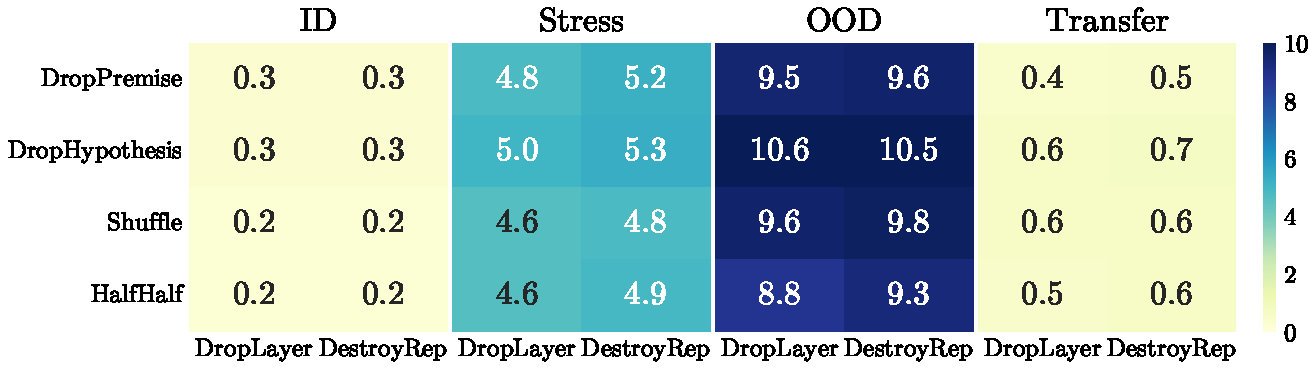
\includegraphics[width=0.5\textwidth]{figure/two_aug.pdf}
    \vspace{-20pt}    
    \caption{Debiasing performance with different combinations of explicit and implicit perturbations. 
    % In this experiment, our model employs one of the explicit perturbations and one of the implicit perturbations. 
    The values indicate relative accuracy % performance
    increase compared to vanilla fine-tuning.}
    % \vspace{-10pt}
    \label{fig:two_aug}
\end{figure}





\paragraph{Debiased Models Are Still Biased}
Our results in Table~\ref{tab:main} and prior reports~\citep{mendelson-belinkov-2021-debiasing,ravichander-etal-2023-bias} show that debiased methods can still be biased. For example, \MASK and \KW show higher levels of biases than \FT
% (without any debiasing objective) 
by 3.7 and 4.2 points on the stress test set~\citep{naik-etal-2018-stress} respectively. These results emphasize the need for modeling multiple types of biases, and highlights the advantages of our approach.
% Similar results have been reported in previous works~\citep{mendelson-belinkov-2021-debiasing,ravichander-etal-2023-bias}.

\paragraph{\OursCL Maintains Generalization across Biases}
Bias in existing methods may be because of their tendency to over-specialize in specific types of biases. \textbf{Table~\ref{tab:subset}} summarizes the performance of debiasing models across different subsets of the stress set. \OursCL achieves the maximum average performance with smaller standard deviation across these subsets, indicating that it does not overfit to specific biases. We attribute such resilience to \OursCL's incorporation of both explicit and implicit perturbations, along with the randomness in implicit perturbations, which allows the model to effectively handle diverse set of biases.

% \begin{table}
% \centering
% \setlength{\tabcolsep}{3.9pt}
% \renewcommand{\arraystretch}{0.9}
% \begin{tabular}{l|c}
% \hline
%     Model & Val. \\
%     \hline
%     Vanilla    & 78.9 \\
%     \MASK      & 70.2 \\
%     \KW        & 73.8 \\
%     \ETEPoe    & 67.4 \\
%     \RUBI      & 69.5 \\
%     \hline    
%     \OursCL    & 54.9 \\
%     \hline
%   \end{tabular}
% \caption{Performance on in-domain validation set of MNLI when feeding shuffled input.}
% \label{tab:un-lang}
% \end{table}


% \subsection{Identify spurious data}
% How to use our model to identify spurious data points in the dataset.

% 1) Look at the output of bias branches

% 2) Look at the attention weights


\begin{table}
\footnotesize
\centering
% \setlength{\tabcolsep}{3.9pt}
% \renewcommand{\arraystretch}{0.9} 
\begin{tabular}{l|lc}
\toprule
\textbf{Model} & \textbf{Param} & \textbf{Time (hr)} \\
\midrule
    \textbf{\FT}   & 110M + 2K & 4.2 \\
    \midrule
    \textbf{\MASK} & + 28M + 2K & 5.3 \\
    \textbf{\KW}   & + 3K & 6.3 \\
    % weak learner & 4.1 \\ 
    \textbf{\ETE}  & + 30K & 5.5 \\
    \textbf{\IE}   & + 50 $\times$ 2K & 7.2 \\
    \textbf{\READ} & + 28M + 2K & 4.9 \\
    \midrule
    \textbf{\OursCL} & + 2 $\times$ 2K & 4.9 \\
    \bottomrule
  \end{tabular}
  \caption{Efficiency of debiasing models on MNLI.}
  \vspace{-20pt}
  \label{tab:eff}
\end{table}

\paragraph{Efficiency}
We evaluate the efficiency of different debiasing methods in terms of number of trainable parameters and training time. 
As \textbf{Table~\ref{tab:eff}} shows,  \OursCL introduces only 4K additional parameters, which is significantly less than 100K in \IE with 50 classifiers, and 28M in \MASK and \READ with an extra weak model. This highlights the efficiency gains from the proposed perturbation operations. Furthermore, \OursCL has the shortest training time. \OursCL achieves these efficiencies without requiring additional training data, operating only by generating diverse views of the input data.


% \subsection{Discussion}\label{sec:discusion}
\paragraph{Perturbation for Data Augmentation}
The explicit perturbation operators proposed in our framework offer a valuable opportunity for data augmentation, leading to improved performances on existing debiasing methods (See Table~\ref{tab:res_aug} in Appendix).


\paragraph{Bias in Different Parts of Inputs}
In our experiments with single explicit perturbations, we find that DropPremise and DropHypothesis lead to similar performances on MNLI, 
% Table~\ref{tab:bias_type} in Appendix~\ref{sec:detail_type_of_bias}, 
showing that there exists dataset bias in premise, potentially as much as those in hypothesis. However, many existing methods tend to overlook biases in the premise in NLI datasets.
%
In addition, biases can often emerge from the interplay of various parts of inputs, rather than a single source. HalfHalf and Shuffle perturbations can capture such types of biases by perturbing the entire inputs. We note that while additional weak learners can potentially capture biases from multiple sources~\citep{utama-etal-2020-towards,sanh2020learning,meissner-etal-2022-debiasing}, their effectiveness  is likely limited by the capabilities of the weak models. 
Our approach addresses dataset biases through a multiview approach to bias, which leads to a more robust debiasing process.






% \paragraph{Connection to other methods} Several existing debiasing methods can be viewed as special cases of the proposed framework. The approaches presented in~\cite{karimi-mahabadi-etal-2020-end,clark-etal-2019-dont,sanh2020learning} can be seen as applying our explicit perturbation DropPremise and employing PoE as the fusion technique. Similarly, the approaches described in~\citep{ghaddar-etal-2021-end,sanh2020learning,meissner-etal-2022-debiasing} align with the application of our implicit perturbation ``DropLayer'' and the use of PoE as the fusion technique. In addition, the approach in~\citep{utama-etal-2020-towards}, which employs an under-trained model as a weak learner, can be seen as the implicit perturbation DestroyRep within our framework.
%
% Finally, compared to debiasing contrastive learning (DCT)~\citep{lyu2023featurelevel}, the normal distribution across classes serves as the positive example for biased inputs and negative example for intact input in our framework.

% \paragraph{Broad applicability of our framework}
% Our framework can be applied to a broad range of tasks. 
% Both the perturbations and the contrastive objective are task-agnostic, making our method applicable to various NLP tasks. For example, in case of single sentences in tasks like sentiment analysis, our method can be leveraged by implementing $\mathcal{P}_{Sub}$, which involves dropping part of the input sentence. This flexibility set our framework apart from existing debiasing methods, which often lack such adaptability or may be confined to specific model architectures. 
% %
% In addition, our framework is not limited to Transformer-based models. For example, debiasing mask~\cite{meissner-etal-2022-debiasing} prunes model parameters except those pertaining to embedding and classifier layer. Our framework is not constrained by this restriction. This means that it can be applied to various tasks, including knowledge graph embedding in which trainable parameters contain only embeddings, such as TransE~\citep{NIPS2013_1cecc7a7}, in which relationships between entities is interpreted as translations operating on the low-dimensional embeddings of the entities.

% as they are mainly designed to debias NLI tasks. \citet{karimi-mahabadi-etal-2020-end,clark-etal-2019-dont} are restricted by the bias in the hypothesis part in sentence-pair tasks.
%



\section{Related Work}

% \paragraph{Dataset bias}
% refers to the spurious correlations between features and labels in datasets. During training, models can learn these shortcut solutions in datasets rather than learning meaningful signals that contribute to the correct predictions for the task. Dataset biases can be specific, such as negation words~\cite{gururangan-etal-2018-annotation} in NLI tasks, or text-only inputs in visual question answering tasks~\cite{cadene2019rubi}. They may also be non-specific or of unknown type, such as biases that exist in weak models~\cite{sanh2020learning}.
%
% Previous work developed stress or out-of-domain test sets to evaluate models against shortcut solutions. For example, \citet{naik-etal-2018-stress} designed a set of rules to generated hard test examples using the original data, e.g., by appending irrelevant text to the data. \citet{mccoy-etal-2019-right} developed a controlled evaluation set called heuristic analysis for NLI systems (HANS) that contains fallible syntactic heuristics, illustrating that strong NLI models fail to achieve good performance on these cases.debiased focal

% The bias identification methods can be broadly classified into two categories, 1) \textit{explicit} identification, and 2) \textit{implicit} identification. 

% On the other hand, \textit{implicit} identification methods aim at identifying bias that we don't know \textit{a priori}. \citep{karimi-mahabadi-etal-2020-end} proposes to use an under-trained model as the bias identifier, while \citep{sanh2020learning} uses a two-layer Bert-tiny model, i.e. an under-parametrized model, as the bias identifier.

% \xhdr{Debias datasets}
% The following work try to debias from the dataset point of view.
\paragraph{Quantifying Bias}
Several works focus on understanding dataset bias and deibasing algorithms, including measurement of bias of specific words with statistical test~\citep{gardner-etal-2021-competency}, identification of biased and generation of non-biased samples with $z$-filtering~\citep{wu-etal-2022-generating}, identification of bias-encoding parameters~\citep{yu-etal-2023-unlearning}, when bias mitigation makes model less or more biased~\citep{ravichander-etal-2023-bias}, bias transfer from  other models~\citep{jin-etal-2021-transferability}, and  representation fairness~\citep{shen-etal-2022-representational}. 


\paragraph{Debiasing with Biased Models} These approaches model shortcuts from datasets, and use biased predictions as a reference to quantify bias in input data. Bias can be \emph{explicit bias} in NLI datasets~\citep{belinkov-etal-2019-dont,clark-etal-2019-dont,karimi-mahabadi-etal-2020-end,utama-etal-2020-mind}, and \emph{implicit bias} detected by weak models~\citep{ghaddar-etal-2021-end,sanh2020learning,meissner-etal-2022-debiasing,utama-etal-2020-towards,meissner-etal-2022-debiasing}. 
% These methods suffer from an incomplete source of biases, which may lead to suboptimal performance.
Ensemble techniques include Product-of-Experts (PoE)~\citep{10.1162/089976602760128018,sanh2020learning,cheng24c_interspeech} which takes element-wise multiplication of the logits, Debiased Focal Loss~\citep{karimi-mahabadi-etal-2020-end} and ConfReg~\citep{utama-etal-2020-mind} which both down-weight predictions based on the confidence of biased models.\looseness-1


\paragraph{Debiased Representations} Existing methods focus on weak-learner guided pruning~\citep{meissner-etal-2022-debiasing}, disentangling robust and spurious representations~\citep{gao-etal-2022-kernel}, 
% using \textit{isotropic} sentence embedding
decision boundaries~\citep{lyu2023feature}, and
attention patterns with PoE~\citep{wang-etal-2023-robust}, 
training biased models with one-vs-rest approach~\citep{jeon-etal-2023-improving}, and amplifying bias in training set with debiased test set~\citep{reif-schwartz-2023-fighting}.

% DCT formulates the debiasing task as learning a robust decision boundary between biased and non-biased examples, by pushing \textit{the closest biased and non-biased examples} away and pull \textit{the farthest biased and non-biased examples} close to each other. 
% READ assume that attention of the \texttt{[CLS]} token is a key source of spuriousness and use a biased model to regularize the attention of the target model.





\paragraph{Fairness and Toxicity} These approaches focus on protected variable such as race. Existing methods spans across counterfactual data augmentation~\citep{zmigrod-etal-2019-counterfactual,dinan-etal-2020-queens,barikeri-etal-2021-redditbias}, comparisons between network architectures~\citep{meade-etal-2022-empirical}, deibasing with counterfactual inference~\citep{qian-etal-2021-counterfactual}, adversarial training~\citep{madanagopal-caverlee-2023-bias}, prompt perturbation~\citep{guo-etal-2023-debias}, data balancing~\citep{han-etal-2022-balancing}, contrastive learning~\citep{cheng2021fairfil}, detecting toxic outputs~\citep{schick-etal-2021-self}, performance degradation incurred by debiasing methods~\citep{meade-etal-2022-empirical}, and benchmarks~\cite{nadeem-etal-2021-stereoset,hartvigsen-etal-2022-toxigen,sun-etal-2022-chapterbreak}. Social debiasing methods may underperform in OOD settings because OOD examples may not contain social stereotypes or biases.

% Compared to these methods, our method targets a broader spectrum of biases.

% CDA that replaces words with bias attributes with their counterparts (e.g. \textit{he} -> \textit{she}) and add the augmented sentences back to the training corpus.
% In contrast to existing debiasing methods that are restricted by the limited types of biases captured, 
% Despite significant progress, existing models often have a single view to dataset biases, often focus on specific types of biases, rely on specialized debiasing objectives, may sacrifice in-domain performance while debiasing, and are often tailored to specific NLP tasks. The present work overcomes these limitations by developing a new debiasing method that effectively models known dataset biases and do not suffer from in-domain performance drop when debiasing.


\section{Conclusion}
We investigate bias mitigation in NLU datasets by 
% introducing a new approach that makes the a learner undecided when encountering biased inputs while being confident when processing full intact inputs. Our debiasing framework 
formulating the debiasing problem within a contrastive learning framework, incorporating explicit and implicit perturbation techniques and introducing undecided learning. Through extensive experiments across a range of NLU tasks, we demonstrate the effectiveness of our method in achieving improved debiasing performance, while maintaining performance on in-domain test sets. We find that existing methods (including ours) are still sensitive to dataset biases, and our experiments show the limitations of these approaches in fully addressing dataset biases. These results necessitate investigating a more systematic evaluation benchmark for debiasing. 
%
Our approach can potentially be improved by
investigating more complex biases~\citep{yao2023large,gandikota2023erasing}, 
exploring alternative training paradigms such as curriculum learning~\citep{bengio2009curriculum,vakil-amiri-2022-generic}, and evaluating robustness to unseen biases~\citep{NEURIPS2023_b0d9ceb3}. 
Beyond NLU, our work can potentially be applied to a broader range of applications~\citep{cheng2024mu,Liu_2024_WACV}.


\newpage
\section*{Limitations}
% Despite significant contributions to mitigating dataset biases, the proposed work has the following limitations: 
% although 
Though our framework outperforms baselines, there is still room for improvement on Stress and OOD test sets.   
In addition, we didn't analyze the generalizability of the approach to other NLP domains or tasks beyond the three tasks used in the experiments.  
% Moreover, the framework introduces additional computational complexity due to the perturbation operations and contrastive learning objective, which may increase the training time. 
% Finally, our experiments are mainly conducted on two encoder models and it's effect on other learner has not been explored. 
\section*{Ethic and Broader Impact Statements}
Our research focuses on mitigating dataset biases in NLP datasets. There are no specific ethical concerns directly associated with this work. However, we acknowledge and emphasize the ethical mindfulness throughout the design, training, and applying the models investigated in this study on any applications.
The broader impacts of our work are in advancing dataset fairness and potentially enhancing decision-making based on data. By addressing biases, we contribute to improving the reliability of NLP datasets and the accuracy and transferability of the models trained using NLP datasets. 

% \section*{Broader Impact Statement}


% \section*{Acknowledgements}


% Entries for the entire Anthology, followed by custom entries
\bibliography{anthology1,anthology2,custom}
% \bibliographystyle{acl_natbib}

\appendix
% \begin{table*}[hbt!]
% \small
% \centering
% % \setlength{\tabcolsep}{3.9pt}
% \begin{tabular}{l|ccccccc}
%     \toprule
%     Model & Antonym & Length   & Negation & Numerical & Spelling & Word  & Average \\ 
%           &         & mismatch &          & reasoning & error    & overlap & \\
%     \midrule
%     Vanilla	   & 48.6 & 78.5 & 52.9 & 36.1 & 76.2 & 60.6 & 58.8 \\
%     \midrule
%     \MASK      & 41.3 & 71.2 & 51.7 & 33.5 & 70.2 & 53.7 & 53.6 \\
%     \KW        & 40.4 & 70.4 & 51.0 & 33.1 & 71.8 & 52.1 & 53.1 \\
%     % \RUBI      &  7.6 & 68.1 & 51.5 & 20.2 & 66.6 & 70.3 & 47.4 \\ 
%     \ETE	   & 47.7 & 77.4 & 52.8 & 36.9 & 75.1 & 56.8 & 57.8 \\
%     \ETEFocal  & 48.4 & 77.1 & 53.2 & 35.2 & 75.8 &	63.7 & 58.9 \\
%     \midrule
%     Ours - $\mathcal{P}=$ DropPremise    & 55.7 & 81.5 & 56.5 & 40.0 & 80.8 & 61.1 & 61.6 \\
%     Ours - $\mathcal{P}=$ DropHypothesis & 55.7 & 81.5 & 56.5 & 40.0 & 80.8 & 61.1 & 61.6 \\
%     Ours - $\mathcal{P}=$ HalfHalf	     & 58.6 & 81.9 & 56.3 & 40.0 & 80.1 & 59.3 & 62.1 \\
%     Ours - $\mathcal{P}=$ Shuffle	     & 58.6 & 81.9 & 56.3 & 40.0 & 80.1 & 59.3 & 62.1 \\
%     Ours - $\mathcal{P}=$ DropLayer	     & 57.1 & 81.5 & 56.5 & 40.2 & 80.6 & 60.7 & 60.3 \\
%     Ours - $\mathcal{P}=$ PerturbRep     & 56.3 & 81.4 & 57.4 & 44.4 & 80.6 & 59.8 & 62.0 \\
%     % \midrule
%     % \OursPoe   & 47.3 & 78.2 & 53.8 & 36.0 & 76.3 & 61.1 & 58.8 \\
%     % \OursFocal & 47.3 & 78.2 & 53.8 & 36.0 & 76.3 & 61.1 & 58.8 \\
%     % \OursCL    & 54.4 & 80.5 & 55.2 & 38.1 & 79.1 & 61.9 & 61.5 \\
%     \bottomrule
% \end{tabular}
% \caption{Detailed results on specific type of biases from stress test set~\citep{naik-etal-2018-stress}.}
% \vspace{-20pt}
% \label{tab:bias_type}
% \end{table*}


\section{Implementation Details}
For all datasets, we train all methods on the BERT-base~\citep{devlin-etal-2019-bert} checkpoint, with a 2e-5 learning rate with linear decay using AdamW~\citep{kingma2014adam} optimizer. The batch size is set to 32. For the baseline models, we follow their papers for the hyperparameter choices. All experiments on done on a single A100 GPU.
% We adopt $\lambda = 0.1$.

% For Contrastive Learning, we adopt $lambda = 0.1$. For Poe and Focal loss, we adopt $lambda = 0.01$.

% \subsection{Settings}
We implement the proposed perturbation as illustrated in Table~\ref{tab:aug_list} by randomly dropping $50\%$ of the tokens from each sentence, dropping all layers after the second layer (3--12), %$k=20\%$), 
and zeroing $m=90\%$ of the elements in the intact representation $f(x_i)$. Each branch-specific MLP consists of two linear layers with a ReLU activation function in between. 
We use $\lambda = 0.1$ in our experiments.


\section{Other Debiasing Objectives}
\label{sec:debias_obj}
The idea of existing debiasing objectives is based on the idea of adjusting the importance of training examples, i.e. their contribution to loss calculation. The importance of examples which the model fails the correctly predict is promoted while the importance of examples which the model correctly predicts is reduced. 

Product-of-Experts (PoE)~\citep{clark-etal-2019-dont,karimi-mahabadi-etal-2020-end,sanh2020learning} is one of the most commonly adopted debiasing objective, which takes dot product of the logits of the main model and the biased models. Debiasing Focal Loss~\citep{karimi-mahabadi-etal-2020-end} down-weights the main model based on how close the logits of the biased models is to 1. Confidence Regularization~\citep{utama-etal-2020-towards} reduced the loss scale of examples with a scaling mechanism.

\section{RoBERTa as Encoder}
We conducted experiments on RoBERTa-base~\citep{liu2019roberta} using the MNLI dataset to evaluate the efficacy of FairFlow more effectively. The results in Table~\ref{tab:roberta} shows that the performance of all models improved using RoBERTa-base as encoder. We also observe comparable gains to BERT as encoder in case of ID and Transfer settings and smaller gains in case of Stress and OOD settings, which can be attributed to the use of a more powerful encoder.


\begin{table*}
\small
\centering
% \setlength{\tabcolsep}{3.9pt}
% \renewcommand{\arraystretch}{0.9} 
\begin{tabular}{l|cccc|cccc|cc}
\toprule
\textbf{Model} & \multicolumn{4}{c|}{\textbf{MNLI} (Acc.)} & \multicolumn{4}{c|}{\textbf{QQP} (F1)} & \multicolumn{2}{c}{\textbf{PGR} (F1)} \\
               & ID   & Stress & OOD & Transfer & ID & Stress & OOD & Transfer & ID & Stress \\ \toprule
    \textbf{\FT}        & 84.4 & 55.8 & 60.7 & 80.1 & 89.1 & 59.3 & 40.8 & 61.8 & 67.1 & 54.3 \\
    \midrule
    \textbf{\MASK}      & 84.7 & 53.6 & 60.8 & 80.5 & 88.3 & 60.2 & 44.7 & 62.1 & 65.4 & 44.6 \\
    \textbf{\KW}        & 83.3 & 53.5 & 60.5 & 80.2 & 87.6 & 61.3 & 45.1 & 62.7 & 63.5 & 42.0 \\
    \textbf{\ETE}       & 83.8 & 57.8 & 66.3 & 80.1 & 89.2 & 58.9 & 42.5 & \underline{63.1} & 63.2 & 50.3 \\
    % \textbf{\RUBI}      & 71.1 & 47.4 & 60.2 & 50.6 & 85.0 & 47.3 & 28.4 & 48.5 & 58.6 & 39.7 \\ 
    \textbf{LWBC}	    & 83.2 & 58.3 & 60.2 & 80.7 & 89.6 & 73.2 & 49.2 & 67.4 & 66.5 & 53.2 \\
    \textbf{\IE}        & 84.5 & 60.1 & 67.2 & 79.8 & 84.6 & 57.3 & \underline{50.6} & 60.5 & 64.8 & 54.6 \\
    \textbf{\READ}      & 79.6 & 58.3 & \textbf{68.4} & 73.0 & 84.5 & 65.8 & 46.7 & 61.7 & 62.6 & 55.0 \\
    \midrule
    \textbf{\OursPoe}   & \underline{84.8} & 62.3 & 67.5 & \underline{81.0} & 89.2 & 77.5 & 48.9 & \underline{63.1} & \underline{67.4} & 55.6 \\
    \textbf{\OursFocal} & \underline{84.8} & \underline{62.8} & \underline{67.9} & 80.9 & \underline{89.6} & \underline{77.8} & 49.2 & \underline{63.1} & \textbf{67.7} & \textbf{56.1} \\
    \textbf{\OursCL}    & \textbf{84.9}    & \textbf{63.6} & \textbf{68.4} & \textbf{81.1} & \textbf{91.8} & \textbf{78.4} & \textbf{51.5} & \textbf{68.3} & \textbf{67.7} & \underline{55.8} \\ \bottomrule
  \end{tabular}
  \caption{Experimental results on three datasets using BERT as the base model. The best performance is in \textbf{bold} and the second best is \underline{underlined}. Note that \IE does not release their code. We tried our best to reproduce the results but failed on HANS, which is 5.2 points lower than the reported 72.4. This is potentially due to implementation and optimization details which the authors did not release.}
  \label{tab:bert}
\end{table*}

\begin{table*}[ht]
\small
\centering
\begin{tabular}{l|cccc|cccc|cc}
\toprule
\multirow{2}{2em}{\textbf{Model}} & \multicolumn{4}{c|}{\textbf{MNLI} (Acc.)} & \multicolumn{4}{c|}{\textbf{QQP} (F1)} & \multicolumn{2}{c}{\textbf{PGR} (F1)} \\
               & ID   & Stress & OOD & Transfer & ID & Stress & OOD & Transfer & ID & Stress \\
    \toprule
    \textbf{\FT}        & 88.1 & 75.3 & 66.4 & 81.0 & 92.2 & 63.5 & 44.7 & 68.3 & 69.3 & 57.1 \\
    \midrule
    \textbf{\MASK}      & 86.5 & 72.7 & 66.9 & 80.7 & 92.5 & 66.1 & 49.1 & 68.7 & 70.2 & 57.5 \\
    \textbf{\KW}        & 88.1 & 74.1 & 67.4 & 79.9 & 93.1 & 66.7 & 50.2 & 68.9 & 71.3 & 58.3 \\
    \textbf{\ETE}       & 88.3 & 72.6 & 69.5 & 80.7 & 92.4 & 66.4 & 50.3 & 68.5 & 70.5 & 57.9 \\
    \textbf{LWBC}       & 84.6 & 69.3 & 66.7 & 81.0 & 91.7 & 63.2 & 43.9 & 67.4 & 70.4 & 54.2 \\
    \textbf{\IE}        & 88.2 & 72.4 & 69.3 & 80.3 & 92.3 & 66.3 & 50.2 & 68.3 & 70.8 & 56.3 \\
    \textbf{\READ}      & 85.3 & 73.5 & 70.3 & 78.5 & 91.4 & 68.1 & 51.0 & 67.8 & 69.3 & 55.7 \\
    \midrule
    \textbf{\OursPoe}   & 88.3 & 76.1 & 70.2 & 81.4 & 92.5 & 66.7 & 50.6 & 68.3 & 70.8 & 58.0 \\
    \textbf{\OursFocal} & 88.2 & 76.7 & 70.3 & 81.4 & 92.7 & 67.8 & 51.3 & 68.7 & 71.1 & 58.3 \\
    \textbf{\OursCL}    & 88.3 & 77.2 & 70.4 & 81.2 & 93.3 & 68.4 & 51.8 & 68.6 & 71.4 & 58.3 \\
    \bottomrule
  \end{tabular}
  \caption{Results using RoBERTa~\citep{liu2019roberta} as the base model. The best performance is in \textbf{bold} and the second best is \underline{underlined}.}
  \label{tab:roberta}
\end{table*}



\begin{table*}
\small
\centering
% \setlength{\tabcolsep}{3.9pt}
% \renewcommand{\arraystretch}{0.9} 
\begin{tabular}{l|cccc|cccc|cc}
\toprule
\multirow{2}{2em}{\textbf{Model}} & \multicolumn{4}{c|}{\textbf{MNLI} (Acc.)} & \multicolumn{4}{c|}{\textbf{QQP} (F1)} & \multicolumn{2}{c}{\textbf{PGR} (F1)} \\
               & ID   & Stress & OOD & Transfer & ID & Stress & OOD & Transfer & ID & Stress \\ \toprule
    \textbf{\FT}        & 80.4 & 54.0 & 52.1 & 75.2 & 84.5 & 67.3 & 57.7 & 65.1 & 56.5 & 54.2 \\
    \midrule
    \textbf{\MASK}      & 79.3 & 52.8 & 51.6 & 73.7 & 83.6 & 67.5 & 57.3 & 74.9 & 56.7 & 53.2 \\
    \textbf{\KW}        & 80.7 & 55.1 & 52.8 & 75.1 & 85.7 & 67.4 & 58.3 & 77.2 & 58.3 & 55.1 \\
    \textbf{\ETE}       & 78.1 & 53.6 & 51.1 & 71.9 & 83.9 & 68.2 & 61.5 & 80.1 & 55.4 & 52.7 \\
    \textbf{LWBC}       & 74.5 & 50.8 & 51.0 & 71.4 & 80.2 & 61.0 & 55.8 & 75.4 & 53.2 & 51.0 \\
    \textbf{\IE}        & 79.7 & 52.9 & 51.8 & 74.3 & 86.1 & 66.9 & 58.2 & 76.2 & 57.1 & 53.8 \\
    \textbf{\READ}      & 77.5 & 52.7 & 51.5 & 73.8 & 85.2 & 66.4 & 63.3 & 75.2 & 57.3 & 52.6 \\
    \midrule
    \textbf{\OursPoe}   & 80.9 & 54.7 & 55.2 & 76.2 & 84.7 & 68.8 & 62.3 & 80.0 & 56.5 & 54.1 \\
    \textbf{\OursFocal} & 81.8 & 55.1 & 54.9 & 75.8 & 86.3 & 68.5 & 64.2 & 80.4 & 57.4 & 55.3 \\
    \textbf{\OursCL}    & 82.2 & 55.6 & 56.1 & 76.7 & 86.3 & 69.3 & 64.7 & 80.4 & 58.6 & 55.8 \\
    \bottomrule
  \end{tabular}
  \caption{Results using GPT-2 as the base model. The best performance is in \textbf{bold} and the second best is \underline{underlined}.}
  \label{tab:gpt2}
\end{table*}


\begin{table}
\small
\centering
% \setlength{\tabcolsep}{3.9pt}
% \renewcommand{\arraystretch}{0.9} 
\begin{tabular}{l|cc}
\toprule
\textbf{Model} & \textbf{Avg. Acc ($\uparrow$)} & \textbf{Std. Acc ($\downarrow$)} \\
    \midrule
    \textbf{\FT}        & 60.1 & 9.3 \\ 
    \midrule
    \textbf{\MASK}      & 58.7 & 6.7 \\ 
    \textbf{\KW}        & 59.3 & 5.9 \\ 
    \textbf{\ETE}       & 60.0 & 6.1 \\
    \textbf{LSWC}       & 59.4 & 5.8 \\ 
    \textbf{\IE}        & 60.1 & 7.3 \\
    \textbf{\READ}      & 60.9 & 5.6 \\ 
    \midrule
    \textbf{\OursPoe}   & 63.8 & 5.7 \\ 
    \textbf{\OursFocal} & \underline{64.3} & \underline{5.2} \\
    \textbf{\OursCL}    & \textbf{64.7} & \textbf{5.1} \\ \bottomrule
  \end{tabular}
  \caption{Average performance and standard deviation on each type of stress test averaged across three architectures. The best performance is in \textbf{bold} and the second best is \underline{underlined}.}
  \label{tab:subset}
\end{table}


\section{Perturbation for Data Augmentation}
The explicit perturbation operators proposed in our framework offer a valuable opportunity for data augmentation. This can be particularly useful in tasks such as NLI. Consider the example $(x_i^p, x_i^h, y_i)$, where $x_i^p$ represents the premise, $x_i^h$ represents the hypothesis, and $y_i$ denotes the label. To augment the dataset, we create additional data samples by applying different perturbation operations, e.g., by dropping the premise: (`', $x_i^h$, not entailment), dropping the hypothesis: ($x_i^p$, `', not entailment), shuffling the data: ($\mathcal{P}_{Irr}(x_i^p)$, $\mathcal{P}_{Irr}(x_i^h)$, not entailment) and dropping parts of the input: ($\mathcal{P}_{Sub}(x_i^p)$, $\mathcal{P}_{Irr}(x_i^h)$, not entailment). 
The augmented examples can be added back to the original dataset to mitigate the effect of bias during fine-tuning and potentially enhance model's generalizability, leading to improved performance on existing debiasing methods (See Table~\ref{tab:res_aug}).

\begin{table*}[ht]
\small
\centering  
\begin{tabular}{l|p{.6cm}p{.6cm}p{.6cm}p{.9cm}}
\toprule
\multirow{2}{2em}{\textbf{Model}} & \multicolumn{4}{c}{\textbf{MNLI} (Acc.)} \\
               & ID   & Stress & OOD & Transfer \\
    \toprule
    \textbf{\FT}         & 84.4 & 55.8 & 60.7 & 80.1 \\
    \textbf{\FT + Aug}   & 84.5 & 59.1 & 61.0 & 81.0 \\
    \midrule
    \textbf{\MASK}       & 84.7 & 53.6 & 60.8 & 80.5 \\
    \textbf{\MASK + Aug} & 85.6 & 55.4 & 62.2 & 81.1 \\
    \textbf{\KW}         & 83.3 & 53.5 & 60.5 & 80.2 \\
    \textbf{\KW + Aug}   & 85.1 & 56.2 & 60.8 & 81.0 \\
    \textbf{\ETE}        & 83.8 & 57.8 & 66.3 & 80.1 \\
    \textbf{\ETE + Aug}  & 84.8 & 61.1 & 66.2 & 80.6 \\
    \textbf{\IE}         & 84.5 & 60.1 & 65.7 & 79.8 \\
    \textbf{\IE + Aug}   & 85.6 & 60.8 & 66.4 & 80.7 \\
    \textbf{\READ}       & 79.6 & 58.3 & 68.4 & 73.0 \\
    \textbf{\READ + Aug} & 79.6 & 58.3 & 69.6 & 77.2 \\
    \bottomrule
  \end{tabular}
  \caption{Performance when applying data augmentation, which effectively improve existing debiasing methods. The best performance is in \textbf{bold}.}
  \label{tab:res_aug}
\end{table*}



% \section{Effect of balancing factor}
% We investigate the effect of the balancing hyperparameter $\lambda$ by varying its value, specifically $0.01, 0.05, 0.1, 0.5, 1$ on MNLI dataset and summarize the results in Table~\ref{tab:hyper}. 

% Our first discovery is that different tasks require different weights between the original branch and the biased branches. For 

% In addition, we find that our contrastive learning approach is more sensitive to the choice of $\lambda$, while other fusion techniques are less sensitive. We attribute this to the fact that in contrastive learning, the gradient of the bias branches is backpropagated to the backbone model. While in the rest of the fusion techniques, the losses of the bias branches do not affect the backbone model. 

% \section{Performance on specific shortcuts}
% \label{sec:detail_type_of_bias}
% We further present the finer-grained performance on different types of biases from the stress test sets~\citep{naik-etal-2018-stress} for MNLI in Table~\ref{tab:bias_type}. Overall, our method can outperform standard fine-tuning by 3.2\% absolute point and other baselines. \MASK~\citep{} and \KW~\citep{}

% We also notice that \RUBI, a visual QA model, has a significantly lower performance than our method and other baselines. Given the fact that \RUBI and \ETEPoe are very similar (\RUBI has an extra sigmoid function before PoE), we attribute this performance drop to  shows difference between multi-modal (VQA) and uni-modal (NLP) datasets. 


% \paragraph{Antonym} In these stress test examples, premise and hypothesis are the same except the verbs are antonyms of each other. Our model $\mathcal{P}=$``Shuffle'' and $\mathcal{P}=$``HalfHalf'' outperforming ``Vanilla'' by 10\% absolute point. The rest of the debiasing methods are even worse than ``Vanilla'', indicating such methods are still biased.

% \paragraph{Length mismatch} In these stress test examples, premise is significantly longer than hypothesis or the other way around. The minimum performance advantage over baselines is 1.9\%.

% \paragraph{Negation} In these stress test examples, negation words are inserted to the verbs in the hypothesis. The minimum performance advantage over baselines is 3.9\%. This shows that our model can be more attentive to details in the input and make better predictions based on that.

% \paragraph{Numerical reasoning} In these stress test examples, models are asked to perform NLI on numerical statements. The minimum performance advantage over baseline is 3.9\% absolute point.

% \paragraph{Spelling error} In these stress test examples, some words are mis-spelled, which may result in `<UNK>' tokens in the vocabulary. The minimum performance advantage over baseline is 4.9\% absolute point. This highlights that our model does not rely on specific words in the sentence to make predictions and is robust to spelling errors.

% \paragraph{Word overlap} In these stress test examples, premise and hypothesis have a large portion of lexical overlap. The minimum performance advantage over baselines is 1.9\%.




\end{document}
